\documentclass{report}
\usepackage{listings}
\usepackage[margin=1.0in]{geometry}
\usepackage{graphicx}
\usepackage{hyperref}
\usepackage{amsmath}
\hypersetup{colorlinks=true}
\usepackage[document]{}
\title{EECE.5200 - Homework 7}
\author{Travis Kessler}
\date{3 May 2021}
\begin{document}
	\maketitle
	\newpage

	\lstset{frame=lines}

	\section*{Accessing Source Code}
	
	Source code is available at: \href{https://github.com/tjkessler/eece5200/tree/main/hw7}{https://github.com/tjkessler/eece5200/tree/main/hw7}

	\textit{}

	\section*{Results}
	
	Figure 1 displays the output of running "./a.out" following the execution of "./E" or "./EMAC". No additional figures are included, as the majority of outputs for this program are auditory and/or are in real-time. It is encouraged that the reader execute the program themselves.
	
	\begin{figure}[!ht]
		\centering
		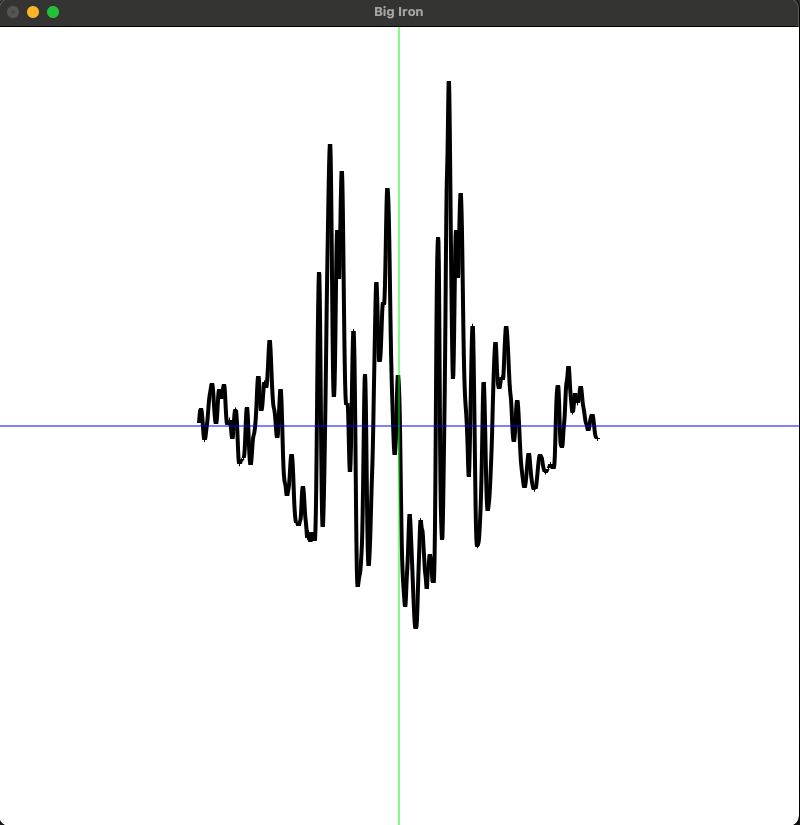
\includegraphics[scale=0.5, trim={0 0.05cm 0 0.0cm}, clip]{figures/res.png}
		\caption{Signal X versus time of "music.wav" during playback}
	\end{figure}

\newpage

	\begin{thebibliography}{99\kern\bibindent}
	
	\bibitem{hwref}
	Thompson, C.
	\textit{University of Massachusetts Lowell Department of Electrical and Computer Engineering 16.520 Computer Aided Engineering Analysis Problem Set 7}.
	Retrieved May 3, 2021, from http://morse.uml.edu/Activities.d/16.520/S2021.d/ps7.pdf
	
	\end{thebibliography}

\end{document}